\documentclass[11pt]{article}
\usepackage[letterpaper,margin=1in]{geometry}
\usepackage{amsmath,amsbsy,amsfonts,amssymb,amsthm,commath}
\usepackage[round]{natbib}
\usepackage{hyperref}
\usepackage{graphicx}
\usepackage{float}
\usepackage{courier}

% math font macros

\def\ddefloop#1{\ifx\ddefloop#1\else\ddef{#1}\expandafter\ddefloop\fi}
% Blackboard fonts: \bbA, \bbB, ...
\def\ddef#1{\expandafter\def\csname bb#1\endcsname{\ensuremath{\mathbb{#1}}}}
\ddefloop ABCDEFGHIJKLMNOPQRSTUVWXYZ\ddefloop
% Calligraphic fonts: \cA, \cB, ...
\def\ddef#1{\expandafter\def\csname c#1\endcsname{\ensuremath{\mathcal{#1}}}}
\ddefloop ABCDEFGHIJKLMNOPQRSTUVWXYZ\ddefloop
% Bold fonts (for vectors, matrices, etc.): \vA, \vB, ..., \va, \vb, ...
\def\ddef#1{\expandafter\def\csname v#1\endcsname{\ensuremath{\boldsymbol{#1}}}}
\ddefloop ABCDEFGHIJKLMNOPQRSTUVWXYZabcdefghijklmnopqrstuvwxyz\ddefloop
% Bold fonts (for vectors, matrices, etc.): \valpha, \vbeta, ...,  \vGamma, \vDelta, ...,
\def\ddef#1{\expandafter\def\csname v#1\endcsname{\ensuremath{\boldsymbol{\csname #1\endcsname}}}}
\ddefloop {alpha}{beta}{gamma}{delta}{epsilon}{varepsilon}{zeta}{eta}{theta}{vartheta}{iota}{kappa}{lambda}{mu}{nu}{xi}{pi}{varpi}{rho}{varrho}{sigma}{varsigma}{tau}{upsilon}{phi}{varphi}{chi}{psi}{omega}{Gamma}{Delta}{Theta}{Lambda}{Xi}{Pi}{Sigma}{varSigma}{Upsilon}{Phi}{Psi}{Omega}{ell}\ddefloop

% other macros

\newcommand\ip[1]{\langle #1 \rangle} % inner product
\newcommand{\E}{\ensuremath{\mathbb{E}}} % expectation
\renewcommand{\P}{\ensuremath{\mathbb{P}}} % probability
\newcommand{\var}{\ensuremath{\operatorname{var}}} % variance
\newcommand{\vol}{\ensuremath{\operatorname{vol}}} % volume
\newcommand{\unitball}[1][d]{\ensuremath{B^{#1}}} % unit ball
\newcommand{\unitsphere}[1][d-1]{\ensuremath{S^{#1}}} % unit sphere
\newcommand{\logmgf}[1]{\ensuremath{\psi_{#1}}} % log mgf
\newcommand{\Normal}{\ensuremath{\operatorname{N}}} % normal distribution

% environments

\newtheorem{theorem}{Theorem}
\newtheorem{lemma}{Lemma}
\theoremstyle{definition}
\newtheorem{problem}{Problem}
\newenvironment{solution}{\noindent\emph{Solution.}}{\hfill$\square$}

%-------------------------------------------------------------------------------
% define my own command:
\newcommand\tab[1][1cm]{\hspace*{#1}}

\usepackage{listings} %For code in appendix
  \lstset{language=Java, numbers=left, showspaces=false, %Set code style
    showstringspaces=false, tabsize=2, breaklines=true}



\begin{document}

%-------------------------------------------------------------------------------
\begin{center}
\Large{} 
\textbf{CSORW4231 HOMEWORK 6} \\
\normalsize{}
Due Mon, Apr 24\\
\large{Jun Hu \\
\textbf{(jh3846)}} \\ 
------------------------------------------------------------------------------------------------------------------
\end{center}
%-------------------------------------------------------------------------------

\begin{problem}
\large{Exercise 22.2-6 and 22.2-7 on Page 602.}
\end{problem}

\begin{solution}
\begin{enumerate}
    \item[\textbf{22.2-6}] As shown in Figure 1. We run BFS on $G$:\\
    \tab If $v_1$ is first explored, it will be first dequeued thereafter explore $v_3,v_4$, so $v_2$ will not explore them.\\
    \tab If $v_2$ is first explored, it will be first dequeued thereafter explore $v_3,v_4$, so $v_1$ will not explore them.\\
    \tab So if one of the $v_1, v_2$ explore one of the $v_3,v_4$, and another one of the $v_1,v_2$ can explore the other one of the $v_3,v_4$, this graph $G_{\pi}$ will certainly not produced by BFS.
    \begin{figure}[htbp]
  \centering
  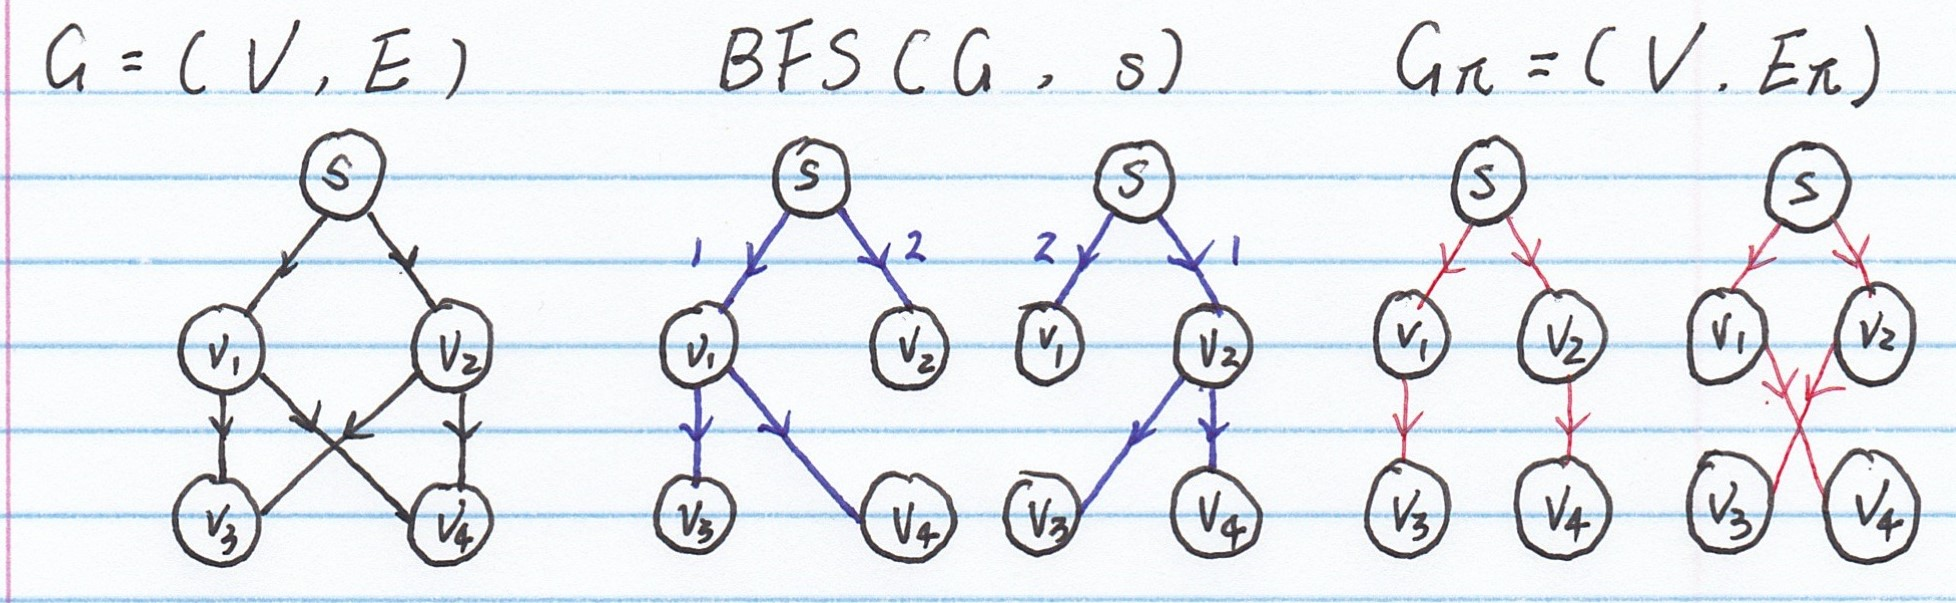
\includegraphics[width=0.8\textwidth]{/Users/vibrioh/Pictures/HW6_1}
  \caption{Graphs of 22.2-6}
  \label{fig:shapes}
\end{figure}
    


 \item[\textbf{22.2-7}] \tab We can look the $n$ professional wrestlers as $n$ vertexes $\in V$, and the $r$ pairs rivalries as $r$ edges $\in E$. So the problem will become whether we can color each vertex with either 'babyface' or 'heel' such that no edge with two vertexes that are colored identically. The algorithm can be as follow:\\
  \tab ($n$ vertexes(wrestlers) $\in V$, $r$ edges(pairs of rivalry) $\in E$, s.t. undirected graph $G = (V, E)$ and $G' \subseteq G$, s.t. $G'$ is all-connected)\\ \\
 \textbf{BFS-COLOR}($G$)\\
 for each $G'$:\\
 \tab run BFS($G',s$) as needed to get all the distance $d$ of vertexes from $s$\\
 \tab color `$babyface$' for all $d$ is odd number\\
 \tab color `$heel$' for all $d$ is even number\\
 \tab for each ($(u,v) \in E$):\\
 \tab \tab if $u.color = v.color$:\\
 \tab \tab \tab return `NO SOLUTION'\\
return colors in $G$\\ \\
\tab \textbf{Correctness}: Running BFS ensures all vertexes are covered. Coloring by odd and even number ensures all vertexes has a different color one after another by the levels of BFS exploring. If the algorithm returns `NO SOLUTION', meaning there exists an edge with same color -- that is two wrestlers are the same role while they are a pair of rivalry. In another word, if there exists an odd circle of vertexes, by observation, there is no way we can color two different colors for all edges. This is the circumstance that no matter how we try, we can not solve the problem. Because we always check the edges for different colors, so when this circumstance is there, we can check it out and return the correct conclusion 'NO SOLUTION'. On the other hand, if all checks pass and no violation on coloring, the return coloring meaning we have designated all wrestlers and any pair of rivalry contains two roles -- `babyface' and `heel'.\\
\tab \textbf{Running time}: BFS takes $O(n+r)$. Coloring takes $O(n)$ because there is $n$ vertexes. Checking takes $O(r)$ because there is $r$ edges. To sum up, the algorithm takes $O(n+r)$. 
 
 



    
\end{enumerate}

\end{solution}

\newpage

%-------------------------------------------------------------------------------

%-------------------------------------------------------------------------------

\begin{problem}
Exercise 22.2-8 on Page 602: Diameter of a tree. (Aim for a linear-time algorithm.)
\end{problem}

\begin{solution}
\begin{enumerate}

    \item[\underline{Algorithm}] $s \in V$, run BST($T, s$) to find the last explored vertex $x$, run BST($T, x$) to get the last explored vertex $y$, $d(x,y)$ is the diameter.


 \item[\underline{Correctness}] \tab First of all, the graph is a tree, which means from one vertex to another vertex, there is one and the only one path, otherwise, there will be a circle in the graph, the graph can not be a tree.\\
 \tab From \textbf{Theorem 22.5 (\textit{Correctness of breadth-first search})}, for the last explored vertex $y$, $d(x,y)$ is the maximum shortest path from $x$. So if the first time BST($T, s$) return $x$ as one endpoint of the diameter, the $y$ will be another one. So we only need to prove $x$ can be one of the endpoint of the diameter. We denote $d(u,v)$ be the diameter, $P_0$ is the path from $u$ to $v$, $P_1$ is the path from $s$ to $x$,  without loss of generality, we only need to prove $d(u,x) = d(u,v)$. \\
     \begin{figure}[htbp]
  \centering
  \includegraphics[width=0.8\textwidth]{/Users/vibrioh/Pictures/HW6_2}
  \caption{Graphs of 22.2-8}
  \label{fig:shapes}
\end{figure}
\tab As shown in \textbf{Figure 2}:\\
 \tab Case 1, $s$ is on the $P_0$. $d(u,v) = d(u, s) + d(s, v) \leq d(u,s) + d(s,x) = d(u,x) $, on the other hand, by definition, $d(u,v) \geq d(u,x)$. That can only be, $d(u,x) = d(u,v)$.\\
 \tab Case 2, $s$ is not on the $P_0$. There must be a vertex $p$ is on $P_0$, and vertex $q$ is on the $P_1$, s.t., $d(p,q) \geq 0$. $d(s,x) \geq d(s,v)$, which is $d(s,q)+d(q,x) \geq d(s,q) + d(q, p) + d(p,v)$ $\Rightarrow$ $d(q,x) \geq d(q,p) +d(p, v)$, both sides add $d(u, p) + d(p, q)$, s.t., $d(u,x) \geq d(u,v) + 2d(p,q) \geq d(u,v)$. On the other hand , by definition, $d(u,v) \geq d(u, x)$. That can only be, $d(u,x) = d(u,v)$.\\
 \tab To sum up, $x$ can be one endpoint of diameter, so $d(x,y) = d(u, v)$, $d(x,y)$ is the diameter.

 \item[\underline{Running-time}] BFS takes $O(\vert V \vert + \vert E \vert)$, for the tree T= ($V, E$), $\vert E \vert = \vert V \vert - 1$, so the algorithm take $O(\vert V \vert)$ totally.

   
   
  \end{enumerate}
\end{solution}

\clearpage


%-------------------------------------------------------------------------------


%-------------------------------------------------------------------------------

%-------------------------------------------------------------------------------

\begin{problem}
Exercise 22.3-5 (c), 22.3-8 and 22.3-11 on Page 612. (For 22.3-11, you only need to give an example to show that the situation described here is possible. In both 22.3-8 and 22.3-11, the examples are very simple directed graphs.)
\end{problem}

\begin{solution}
\begin{enumerate}

 \item[\textbf{22.3-5(c)}] \tab If $(u,v)$ is a cross edge: one vertex is not an ancestor of the other, by \textbf{Parenthesis theorem}, $[u.d, u.f]$ and $[v.d, v.f]$ are entirely disjoint, that is either $v.d<v.f<u.d<u.f$ or $u.d<u.f<v.d<v.f$. However, if $u.d<v.d$, when $v$ is discovered at $v.d$, it is `while', which indicates a tree edge, by \textbf{White-path theorem}, $v$ is a descendant of $u$, contradiction. So, it can be only $v.d<v.f<u.d<u.f$.\\
 \tab If $v.d<v.f<u.d<u.f$, by \textbf{Parenthesis theorem}, one vertex is not an ancestor of the other, that is $(u,v)$ can only be a cross edge.\\
\tab To sum up, edge $(u,v)$ is a cross edge if and only if $v.d<v.f<u.d<u.f$ .

 \item[\textbf{22.3-8}] 
    \tab As shown in \textbf{Figure 3}, $G$ contains a path from $u$ to $v$, while $s.d<u.d<u.f<v.d<v.f<s.f$, which is $u.d<v.d$, $v$ is not a descendant of $u$.
    
     \item[\textbf{22.3-11}] 
    \tab As shown in \textbf{Figure 3}, $u$ contains incoming and outgoing edges, but $G$ produces a forest containing only $u$.\\
    
        \begin{figure}[htbp]
  \centering
  \includegraphics[width=0.8\textwidth]{/Users/vibrioh/Pictures/HW6_3}
  \caption{Graphs of 22.3-8 and 22.3-11}
  \label{fig:shapes}
\end{figure}
    
\end{enumerate}

\end{solution} 

\newpage

%-------------------------------------------------------------------------------

%-------------------------------------------------------------------------------

\begin{problem}
Exercise 22.4-2 on Page 614 and Exercise 22.5-7 on Page 621.
\end{problem}

\begin{solution}

\begin{enumerate}

 \item[\textbf{22.4-2}] 
 \tab We can use TOPOLOGICAL-SORT to obtain the linked list and count for every diverged route from $s$ to the $t$.\\ \\
 \textbf{SIMPLE-PATH-NUMBER}($G,s,t$)\\ 
 list = \textbf{TOPOLOGICAL-SORT}($G$)\\
 initiate count[$u$] = 0 for all vertexes in the list\\
 set count[$s$] = 1\\
 for each $v$ in the list:\\
 \tab if $v \neq t$:\\
 \tab \tab for each $w$ in the adjacent[$v$]:\\
 \tab \tab \tab count[$w$] = count[$w$] + count[$v$]\\
 \tab else break\\
 return count[$t$]\\
 
 \tab \textbf{Correctness}: In the DAG, after TOPOLOGICAL-SORT, the list contains ordered vertexes with paths from $s$ to $t$. At the beginning, because all the count[$v$] for the vertexes before $s$ is initialized as $0$, so count[adjacent$v$] will keep $0$, and the `simple path' can not start before $s$ either. When $s$ encountered, because count[$s$] = $1$, if no additional precede neighbor, the count[adjacent$v$] won't increase. But for each additional precede neighbor, count[adjacent$v$] will increase $1$, and the paths to the current vertexes obviously also increased $1$ for each precede neighbor. So when this count[adjacent$v$] pass through $t$, the algorithm terminates and return count[$t$] correctly. If $t$ is ahead of $s$, or $t$ is behind $s$ but not reachable by $s$, accumulated count[$s$] will not pass to $t$, so the algorithm also terminates with count[$t$] = $0$ correctly. \\
 \tab \textbf{Running-time}: TOPOLOGICAL-SORT takes $O(\vert V \vert + \vert E \vert)$, in the `for' loop for counting operation, it is actually counting neighbors -- the neighbor is depends on edges, each edge is counted at the most twice. In the worst case, it is $O(\vert E \vert)$. So the algorithm totally takes $O(\vert V \vert + \vert E \vert)$.
 
 \item[\textbf{22.5-7}] \tab for each strongly-connect-component as a vertex, the component DAG graph $G^{SCC}$, if it is semiconnected, then the original $G$ is semiconnected (the question didn't define one vertex graph G):\\ \\
 \textbf{IS-SEMICONNECTED}($G$)\\
 run \textbf{STRONGLY-CONNECTED-COMPONENTS}($G$)\\
 construct component graph using $SCC$, s.t. $G^{SCC} = (V^{SCC}, E^{SCC})$\\
 list = \textbf{TOPOLOGICAL-SORT}($G^{SCC}$)\\
 for $i$ from $1$ to len[list]$-1$ (if len[list]$ > 1$):\\
 \tab if list[$i$] and list[$i+1$] have NO edge:\\
 \tab \tab return `NOT SEMICONNECTED'\\
 return `SEMICONNECTED'\\
\\
\tab \textbf{Correctness}: After we run STRONGLY-CONNECTED-COMPONENTS, vertexes inside each SCC are reachable both sides. The $G^{SCC}$ is a DAG graph, so after we run TOPOLOGICAL-SORT, the $V^{SCC}$ now in an order of a linked list. If there is an edge for each list[$i$] and list[$i+1$], then apparently $G^{SCC}$ is semiconnected because each vertex is in the ordered chain, linear linked, to the same direction. As a result, the original $G$ is semiconnected because of the property of SCC. On the other hand, if $G^{SCC}$ is semiconnected, the TOPOLOGICAL-SORT must return a linked chain that each pair of list[$i$] and list[$i+1$] has an edge, otherwise there is no path for list[$i$] and list[$i+1$] to be reachable for each other, because they are forked to the same direction, no way back. Because SCC is always all reachable inside, if $G$ is not semiconneted, then $G^{SCC}$ is not semiconnected, then the TOPOLOGICAL-SORT return the list is not linear linked, the algorithm will return `NOT SEMICONNECTED' correctly.

\tab \textbf{Running-time}: STRONGLY-CONNECTED-COMPONENTS takes $O(\vert V \vert + \vert E \vert)$. $G^{SCC}$ construction takes $O(\vert V \vert + \vert E \vert)$. TOPOLOGICAL-SORT takes $O(\vert V \vert + \vert E \vert)$ in the worst case $G^{SCC} = G$. For loop takes $O(\vert V \vert + \vert E \vert)$ to scan through all adjacency once. To sum up, the algorithm takes $O(\vert V \vert + \vert E \vert)$.
    
\end{enumerate}


\end{solution}

\newpage
%-------------------------------------------------------------------------------

%-------------------------------------------------------------------------------

%-------------------------------------------------------------------------------

\begin{problem}
Problem 22-2 on Page 621 from (a) to (f): Articulation points and bridges. Note that this problem has 20 points.
\end{problem}

\begin{solution}
\begin{enumerate}

 \item[\textbf{a.}] \tab On one hand, assume the root of $G_{\pi}$ is an articulation. So if we remove the root, there should be at least two components. If the root of a DFS tree has only on child, then there will be only one component produced. So the root has to have at least two children to have at least two components to be an articulation point. \\
 \tab On the other hand,  assume the root of $G_{\pi}$ has at least two children. So if we remove root, by the \textbf{Theorem 22.10} edges in DFS tree are either tree edges or back edges. The children of the root must become disconnected. So the root with at least two children must be an articulation point.
 
  \item[\textbf{b.}] \tab On one had, assume the nonroot vertex $v$ has a child $s$ such that there is no back edge from $s$ or any descendant of $s$ to a proper ancestor of $v$, $v.ancestors$. By the \textbf{Theorem 22.10} edges in DFS tree are either tree edges or back edges. So without $v$, the only tree edge and back edge are cut off, $s$ and $s.children$ have no way to reach $v.ancestors$, which means the two components are disconnected, that is, $v$ is an articulation point.\\
  \tab On the other hand, if assume the nonroot vertex $v$ has a child $s$ such that there are some back edges from $s$ or any descendant of $s$ to a proper ancestor of $v$, $v.ancestors$. Even if $v$ is deleted, there are other back edges for $s$ and $s.children$ to reach $v.ancestors$ -- that is $v$ can not be an articulation point under this circumstance.\\
  
  \item[\textbf{c.}] \tab To compute all vertexes for $v.low$, because $v.d$ is computed during  \textbf{DFS-Visit}, we can easily add this attribute into \textbf{DFS-Visit}($G, u$)\\
  \\
  \textbf{DFS-Visit-Low}($G,u$)\\
  $time = time + 1$\\
  $u.d = time $\\
  $u.low = u.d$ \tab\tab\tab \#\# initialize $u.low$ as $u.d$\\
  $u.color = $ GRAY\\
  for each $v \in G.adj[u]$\\
  \tab if $u.color ==$ WHITE \tab\tab\tab \#\# tree edge\\
  \tab \tab $v. \pi = u$\\
  \tab \tab  \textbf{DFS-Visit-Low}($G,v$)\\
  \tab \tab if $v.low < u.low$: \tab\tab\tab \#\# check for minimum\\
  \tab \tab \tab $u.low = v.low$ \tab\tab\tab \#\# sign for minimum $u.low$\\
  \tab if $u.color ==$ GRAY \tab\tab\tab \#\# back edge\\
    \tab \tab if $v.d < u.low$: \tab\tab\tab \#\# check for minimum\\
      \tab \tab \tab $u.low = v.d$ \tab\tab\tab \#\# sign for minimum $u.low$\\
  $u.color = $ BLACK\\
  $time = time + 1$\\
  $u.f = time$\\
  \\
  \tab \textbf{Correctness}: the algorithm doesn't change anything in \textbf{DFS-Visit}, only for each vertex, checking and signing for the $u.low$ as defined.\\
  \tab \textbf{Running-time}: It takes the same as \textbf{DFS-Visit} because without changing loop and recursion conditions, which is $O(V+E)$. And as an undirected graph, $\vert V \vert - 1 \leq  \vert E \vert  = \binom {\vert V \vert}{2} \leq \vert V \vert ^2 $. The algorithm takes $O(E)$.
  
  
  \item[\textbf{d.}]  \tab From \textbf{c}, we know we can run DFS with \textbf{DFS-Visit-Low}($G,u$) in $O(E)$. Then as shown in \textbf{a}, if the vertex is a root, if it has at least two children, it is an articulation point. As shown in \textbf{b}, for the nonroot vertex $v$, if any $v.child.low \geq v.d$, which means no back edge of this $v.child$ and $v.child.children$ to $v.ancestors$, in this circumstance, there must be a disconnect component produced after deleting $v$, then the nonroot $v$ is an articulation point. The checking for $v.child.low$ takes also $O(E)$ since we compare the vertexes of one edge. So the algorithm takes $O(E)$.
  
  \item[\textbf{e.}] \tab On one hand, if the edge lies in a simple cycle, which means except for the edge, there must be other paths for the other vertexes to be reachable. So if the edge is removed, the cycle may be broke, but the remain component is still connected -- that is, the edge can not be a bridge by definition.\\
  \tab On the other hand, if the edge does not lie in any cycle, which means it is the only way for both sides components of the edge to be connected through the edge's endpoint vertexes, otherwise it forms a cycle. Upon removal, no other path for two sides components to connect --  that is, this edge is a bridge by definition.\\
  
  \item[\textbf{f.}] \tab Considering a bridge does not lies in any cycle, so for the bridge edge ($v, v.child$), $v.child$ and $v.child.children$ should not exist a back edge and subsequently form a cycle, and they can not be equal since lying in different biconnected components, so $v.child.low > v.d$; on the other hand, if $v.child.low > v.d$, no other back edge to $v.ancestors$, there is no cycle for $v$ and $v.child$, and $v$ and $v.child$ lie in different biconnected components, ($v, v.child$) is a bridge. So we can run DFS with \textbf{DFS-Visit-Low}($G,u$) in $O(E)$, check for the vertexes that exists $v.child.low > v.d$, such $(v, v.child)$ is a bridge. The checking takes also $O(E)$ since we check edges. So this algorithm will take $O(E)$.



\end{enumerate}


\end{solution}







\end{document}